\documentclass[11pt]{article}
\usepackage[utf8]{inputenc}
\usepackage{fullpage}
\usepackage{amsmath}
\usepackage{amsthm}
\usepackage{amssymb}
\usepackage{dsfont}
\usepackage{graphicx}
\usepackage{enumerate}
\usepackage[margin=1in]{geometry}
\usepackage{multicol}
\usepackage{tikz}
\usepackage{xcolor}
\usepackage{float}
\usepackage{pgfplots}
\usepackage{pdfpages}
\usepackage{natbib}
\usepackage{bbold}
\usepackage{booktabs}
\usepackage{caption}
\usepackage[hang,flushmargin]{footmisc} % gets rid of indentation in footnote
\usepackage[parfill]{parskip}
\usepackage{listings}
\usepackage[space]{grffile} % pkg for allowing spaces in image file names
\usepackage{color}
\definecolor{mygreen}{RGB}{28,172,0} % color values Red, Green, Blue
\definecolor{mylilas}{RGB}{170,55,241}

\pgfplotsset{compat=1.16}

\usepackage{color}
\usepackage{hyperref}
\hypersetup{
    colorlinks=true, % make the links colored
    linkcolor=blue, % color TOC links in blue
    urlcolor=red, % color URLs in red
    citecolor=black,
    linktoc=all % 'all' will create links for everything in the TOC
}

\title{\vspace{-1.5cm}Assignment 1 Writeup}
\author{Yixin Sun}
\date{\today}
\begin{document}

\maketitle

\section{Figure 1}
\begin{figure}[h]
    \centering
    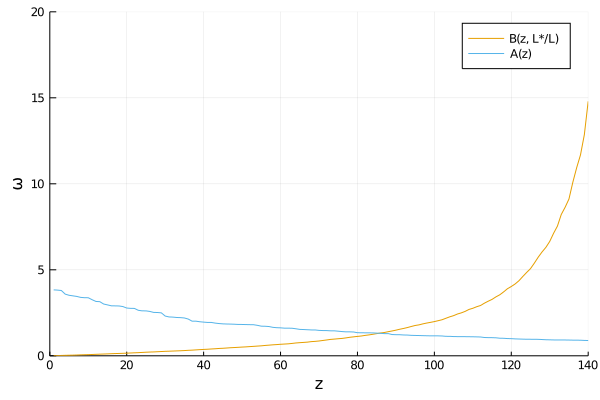
\includegraphics[width=0.8\textwidth]{fig1.png}
\end{figure}

The code to replicate this is the first section in DFS1977master.jl. 

\section{Solving for Equilibrium}
\begin{table}[H]
    \centering
    \caption{Equilibrium $\omega$ and Specialization}
    \begin{tabular}{ccc}
$Var$ & $g1$ & $g9$\\
$z^{star}$ & $86.0$ & $72.0$\\
$z$ & $86.0$ & $95.0$\\
$\omega$ & $1.306$ & $1.314$\\
\end{tabular}

\end{table}

The function that solves for the equilibrium values is in DFS1977solver.jl. DFS1977master.jl calls this function to generate the values for Table 1, taking the ''DFS1977\_example\_a.txt" and ''DFS1977\_example\_b.txt" files as inputs. 

\section{Calculating Welfare}
From class, we can calculate welfare using:
\begin{align*}
    \ln (U / L)=\ln w-\int_{0}^{1} b(z) \ln p(z) d z
\end{align*}

Reformulating this equation, setting $w = 1$ and $L = L^* = 1$, Home's welfares in autarky and trade are:
\begin{align*}
    \ln (U^a / L) &=\ln w-\int_{0}^{1} b(z) \ln (a(z) w L) d z \\
    &= -\int_{0}^{1} b(z) \ln (a(z)) d z \\
    \ln (U^t / L) &= \ln w-\int_{0}^{\bar{z}} b(z) \ln (w a(z) ) d z-\int_{\bar{z}}^{1} b(z) \ln \left(a^{*}(z) \frac{w^{*} L^{*}}{g}\right) d z \\
    &= -\int_{0}^{\bar{z}} b(z) \ln (a(z)) d z-\int_{\bar{z}}^{1} b(z) \ln \left(\frac{a^{*}(z) }{\bar{\omega}g}\right) d z
\end{align*}

Similarly, Foreign's welfares are:
\begin{align*}
    \ln (U^{* a} / L^*) &=\ln \left(\frac{1}{\bar{\omega}}\right)-\int_{0}^{1} b(z) \ln (w* a^*(z)) dz \\
    \ln (U^{* t} / L^*) &= \ln \left(\frac{1}{\bar{\omega}}\right) -\int_{\bar{z}^*}^{1} b(z) \ln \left(\frac{a^*(z)}{\bar{\omega}}\right) d z-\int_{0}^{\bar{z}^*} b(z) \ln \left(\frac{a(z) }{g}\right) d z
\end{align*}

\begin{table}[H]
    \centering
    \caption{Welfare: $ln(U/L)$}
    \begin{tabular}{@{}lll@{}}
    \toprule
    Var               & $g = 1$ & $g = 0.9$ \\ \midrule
    Home - Autarky    & 0.421   & 0.421     \\
    Home - Trade      & 0.527   & 0.487      \\
    Foreign - Autarky & 0  & 0    \\
    Foreign - Trade   & 0.26   & 0.202   \\ \bottomrule
    \end{tabular}
\end{table}

DFS1977solver.jl has another function that computes the log welfare for Home and Foreign, in both autarky and trade equilibriums. The function is called DFS1977welfare. 

\section{Volume of Trade and Gains from Trade}
To calculate the amount traded, we want to find 
\begin{align*}
    Volume =\int_{0}^{\bar{z}^{*}} p(z) c(z) d z + \int_{\bar{z}}^{1} p(z) c(z) d z
\end{align*}

We have that $b(z) = \frac{p(z)c(z)}{wL}$ and $w = 1$, so we can write 
\begin{align*}
    Volume = \int_{0}^{\bar{z}^{*}} b(z) w^* L^{*} d z+\int_{\bar{z}}^{1} b(z) L d z
\end{align*}

DFS1977solver.jl has another function that computes the volume traded, called DFS1977volume. 

Table 3 presents economies with different $b(z)$ schedules that generate the same volume of trade. We see that these three economies differ in equilibrium values and specialization patterns, as well as gains from trade. We cannot infer a one to one relationship here between gains from trade and volume when the differences are generated by shifts in $b(z)$. 

\begin{table}[H]
    \centering
    \caption{Changing $b(z)$}
    \begin{tabular}{@{}llll@{}}
\toprule
Var             & Economy 1 & Economy2 & Economy 3 \\ \midrule
$\bar{z}$       & 72        & 75       & 67        \\
$\bar{z}^*$     & 95        & 102      & 90        \\
$\omega$        & 1.314     & 1.28     & 1.364     \\
Volume          & 0.734     & 0.734    & 0.734     \\
Gains - Home    & 0.066     & 0.068    & 0.073     \\
Gains - Foreign & 0.475     & 0.449    & 0.527     \\ \bottomrule
\end{tabular}

\end{table}


I was not able to generate similar trade volumes by shifting the $A(z)$ schedule while holding $b(z)$ constant. Table 4 presents examples of economies with different shocks to $A(z)$. The first column is the original economy from the previous sections. The second column is a uniform increase in Foreign technology, where $a^*$ is multiplied by $1.5$. The third column is a uniform increase in Home technology, where $a$ is multiplied by $1.5$. If we do not observe autarky prices, we see that changes in the volume of trade has different effects on gains from trade between Home and Foreign. The Home gains seem correlated with volume while the Foreign gains seem negatively correlated with volume. 
\begin{table}[H]
    \centering
    \caption{Changing $A(z)$}
    \begin{tabular}{llll}
\hline
Var             & Economy1 & Economy4 & Economy5 \\ \hline
$\bar{z}$       & 72       & 79       & 61       \\
$\bar{z}^*$     & 95       & 108      & 86       \\
$\omega$        & 1.314    & 1.854    & 0.967    \\
Volume          & 0.816    & 0.632    & 0.951    \\
Gains - Home    & 0.066    & 0.046    & 0.106    \\
Gains - Foreign & 0.202    & 0.233    & 0.159    \\ \hline
\end{tabular}

\end{table}

\end{document}
